\documentclass[aspectratio=169,10pt]{beamer}
\usetheme{metropolis}
\usepackage{graphicx}
\usepackage{tikz}
\usetikzlibrary{decorations.pathreplacing}
\graphicspath{{../reports/figures/}}

\title{Does WTI Crude Oil Have Intraday Momentum?}
\subtitle{A post-2020 replication of Baltussen, Da, Lammers and Martens (2021)}
\author{Gabriella Wiem \and Jiayi Chen \and Ethan Huang}
\institute{FINM 37000, Group 3}
\date{}

\begin{document}
\maketitle
\addtocounter{framenumber}{1}

\begin{frame}[t]{What we test}
  \textbf{Claim (BDLM 2021):} the market's move from yesterday's close until 30 minutes before today's close predicts the last 30 minutes.
  \begin{itemize}
    \item \textbf{LH}: return 13:00--13:30 Chicago time (what we predict)
    \item \textbf{ROD}: return from previous 13:30 to 13:00 (the predictor)
    \item \textbf{ON} / \textbf{DAY}: ROD split at 08:00 into overnight and daytime parts
    \item \textbf{Slope}: basis points of LH per 1\% of the predictor. Positive is momentum, negative is reversal.
  \end{itemize}
  \textbf{Data:} Databento CME Globex one-minute bars, CL futures, 1,436 trading days, Jan 2021 to Oct 2026. 936 out-of-sample forecasts from Jan 2023.
\end{frame}

\begin{frame}{Timeline of the predictors (Chicago time, not to scale)}
  \centering
  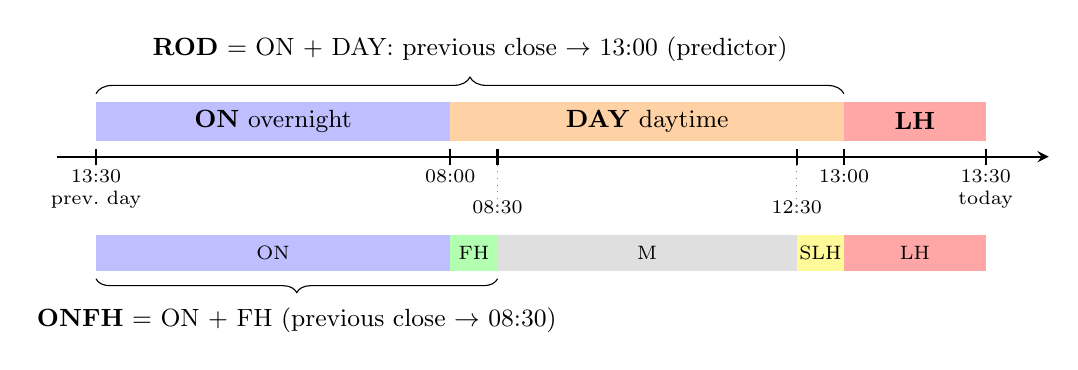
\begin{tikzpicture}[x=1cm,y=1cm,>=stealth]
    \draw[thick,->] (0,0) -- (12.6,0);
    \foreach \x/\l in {0.5/{13:30\\prev.\ day},5/{08:00},10/{13:00},11.8/{13:30\\today}}
      \draw[thick] (\x,-0.1) -- (\x,0.1) node[below=4pt,align=center,font=\scriptsize] {\l};
    \foreach \x/\l in {5.6/{08:30},9.4/{12:30}}
      \draw[thick] (\x,-0.1) -- (\x,0.1) node[below=15pt,font=\scriptsize] {\l};
    \foreach \x in {5.6,9.4} \draw[gray,dotted] (\x,-0.1) -- (\x,-0.75);
    % row 1: our two parts and the target
    \fill[blue!25]   (0.5,0.2) rectangle (5,0.7);
    \fill[orange!35] (5,0.2)   rectangle (10,0.7);
    \fill[red!35]    (10,0.2)  rectangle (11.8,0.7);
    \node[font=\small] at (2.75,0.45) {\textbf{ON} overnight};
    \node[font=\small] at (7.5,0.45)  {\textbf{DAY} daytime};
    \node[font=\small] at (10.9,0.45) {\textbf{LH}};
    \draw[decorate,decoration={brace,amplitude=6pt}] (0.5,0.8) -- (10,0.8)
      node[midway,above=8pt,font=\small] {\textbf{ROD} = ON + DAY: previous close $\to$ 13:00 (predictor)};
    % row 2: the paper's finer pieces
    \fill[blue!25]   (0.5,-1.45) rectangle (5,-1.0);
    \fill[green!30]  (5,-1.45)   rectangle (5.6,-1.0);
    \fill[gray!25]   (5.6,-1.45) rectangle (9.4,-1.0);
    \fill[yellow!40] (9.4,-1.45) rectangle (10,-1.0);
    \fill[red!35]    (10,-1.45)  rectangle (11.8,-1.0);
    \node[font=\scriptsize] at (2.75,-1.225) {ON};
    \node[font=\scriptsize] at (5.3,-1.225)  {FH};
    \node[font=\scriptsize] at (7.5,-1.225)  {M};
    \node[font=\scriptsize] at (9.7,-1.225)  {SLH};
    \node[font=\scriptsize] at (10.9,-1.225) {LH};
    \draw[decorate,decoration={brace,amplitude=5pt,mirror}] (0.5,-1.55) -- (5.6,-1.55)
      node[midway,below=7pt,font=\small] {\textbf{ONFH} = ON + FH (previous close $\to$ 08:30)};
  \end{tikzpicture}

  \vspace{4pt}
  \footnotesize
  \textbf{FH}: first half hour after the 08:00 open. \textbf{M}: 08:30 to 12:30. \textbf{SLH}: 12:30 to 13:00, the second-to-last half hour.\\
  The decision is made at 13:00: every predictor uses prices only up to then. $(1+ON)(1+DAY)=1+ROD$.\\
  13:30 Chicago time (14:30 ET) is the reference close, not the end of the electronic session.
\end{frame}

\begin{frame}{Replication: the paper's regressions}
  Each day $t$, regress the last-half-hour return on a predictor, with an intercept:
  \[
    LH_t = \alpha + \beta\, ROD_t + \varepsilon_t
  \]
  The paper also uses two other versions:
  \begin{align*}
    LH_t &= \alpha + \beta\, ONFH_t + \varepsilon_t\\
    LH_t &= \alpha + \beta_1\, ONFH_t + \beta_2\, M_t + \beta_3\, SLH_t + \varepsilon_t
  \end{align*}
  \small ONFH: overnight plus first half hour (previous close to 08:30). M: 08:30 to 12:30. SLH: 12:30 to 13:00.\\
  \normalsize
  \textbf{Null:} $\beta = 0$ (no predictability). $\beta>0$ is momentum.\\
  We report $\hat\beta$ with Newey-West standard errors (7 lags), plus expanding-window out-of-sample $R^2$ against the historical mean.
\end{frame}

\begin{frame}[t]{Our three new hypotheses}
  \textbf{H1. Overnight vs.\ daytime.}
  \[ LH_t = \alpha + \beta_{ON}\, ON_t + \beta_{DAY}\, DAY_t + \varepsilon_t,
     \qquad H_0:\ \beta_{ON} = \beta_{DAY} \]
  \textbf{H2. Volatility regimes.} $HV_t=1$ if realized variance up to 13:00 is above the 75th percentile of earlier days.
  \[ LH_t = \alpha + \beta_{ON} ON_t + \beta_{DAY} DAY_t + \gamma_{ON}\, ON_t HV_t + \gamma_{DAY}\, DAY_t HV_t + \varepsilon_t \]
  \[ H_0:\ \gamma_{ON}=\gamma_{DAY}=0 \]
  \textbf{H3. Agreement.} $Agree_t = 1$ if $ON_t$ and $DAY_t$ have the same sign.
  \[ LH_t = \alpha + \beta\, ROD_t + \gamma\, Agree_t + \delta\, ROD_t Agree_t + \varepsilon_t,
     \qquad H_0:\ \delta = 0 \]
  Also: the paper's strategy return $\eta_t = \mathrm{sign}(ROD_t)\cdot LH_t$ has the same mean on agree and disagree days.
\end{frame}

\begin{frame}{Finding 1: no intraday momentum in post-2020 CL}
  \centering
  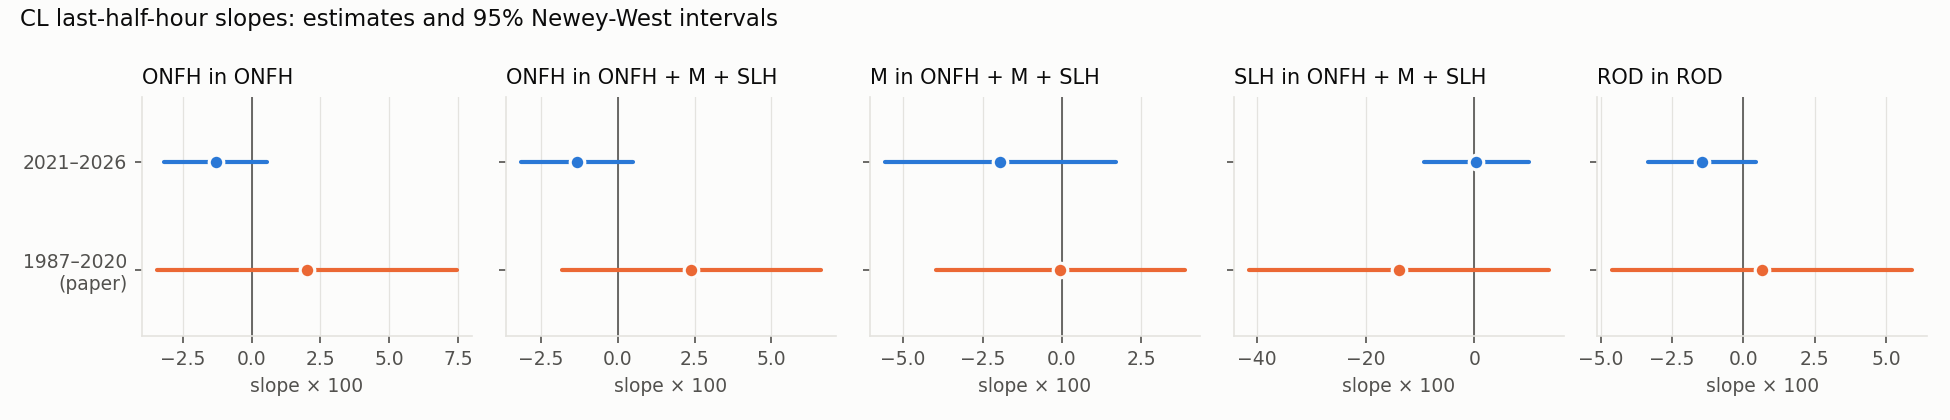
\includegraphics[width=\textwidth]{replication_vs_paper.png}
  \begin{itemize}
    \item ROD slope: $-1.46$, 95\% interval $[-3.35,\,0.43]$. The paper's CL estimate was $+0.67$ ($t=0.25$).
    \item Every post-2020 interval includes zero. The paper's strong results come from other markets and pooled data.
  \end{itemize}
\end{frame}

\begin{frame}{Finding 2: the signal cannot be traded}
  \begin{columns}[T]
    \begin{column}{0.48\textwidth}
      Long if ROD $>0$, short otherwise, over the last half hour.
      \begin{itemize}
        \item Gross: $-1.2$ bp/day (SE 1.3)
        \item Net of USD 15 per round trip: $-3.1$ bp/day, Sharpe $-1.1$
        \item Gross is already negative, so no cost level helps
      \end{itemize}
    \end{column}
    \begin{column}{0.52\textwidth}
      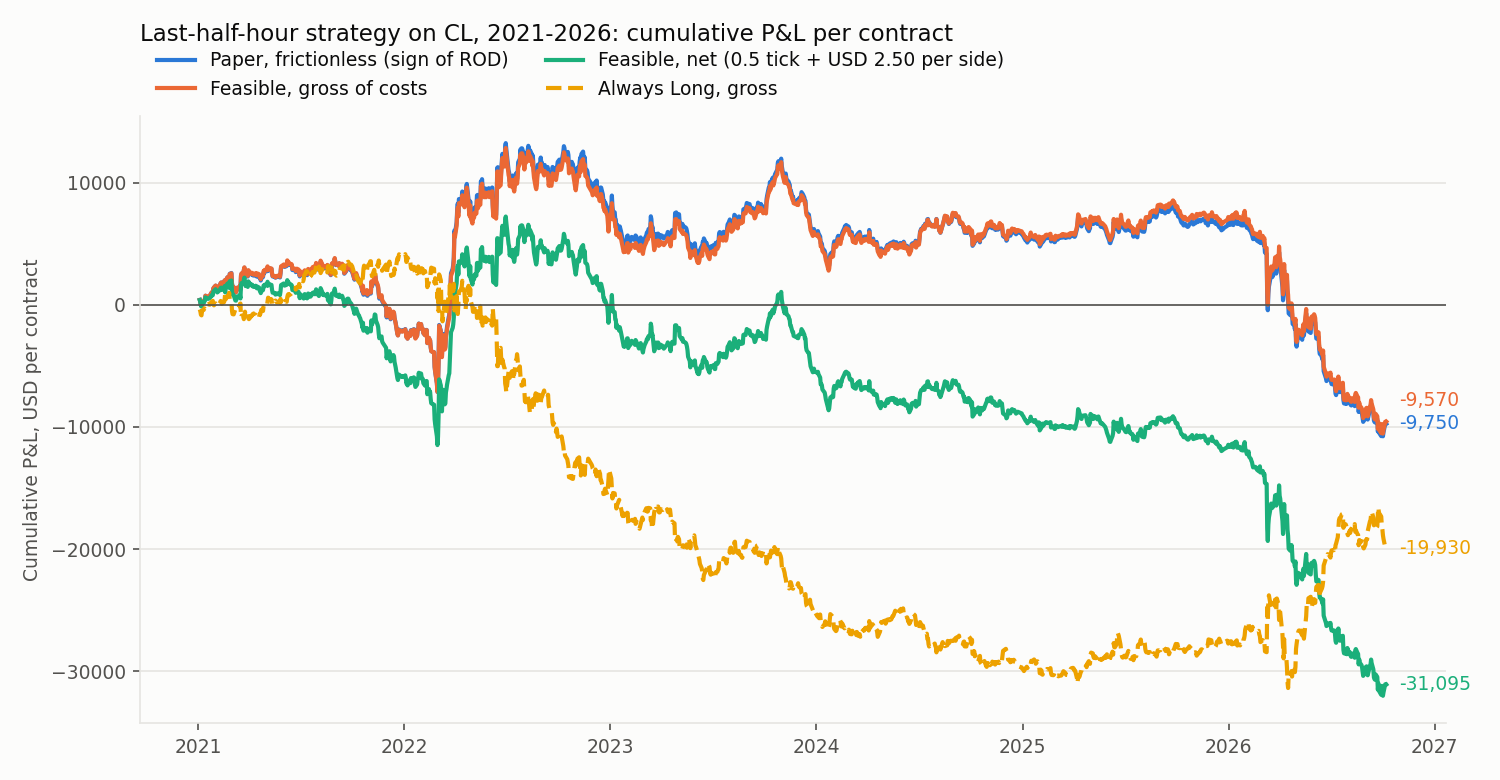
\includegraphics[width=\textwidth]{lh_strategy_cumulative.png}
    \end{column}
  \end{columns}
\end{frame}

\begin{frame}{Finding 3: overnight and daytime do not predict differently}
  \centering
  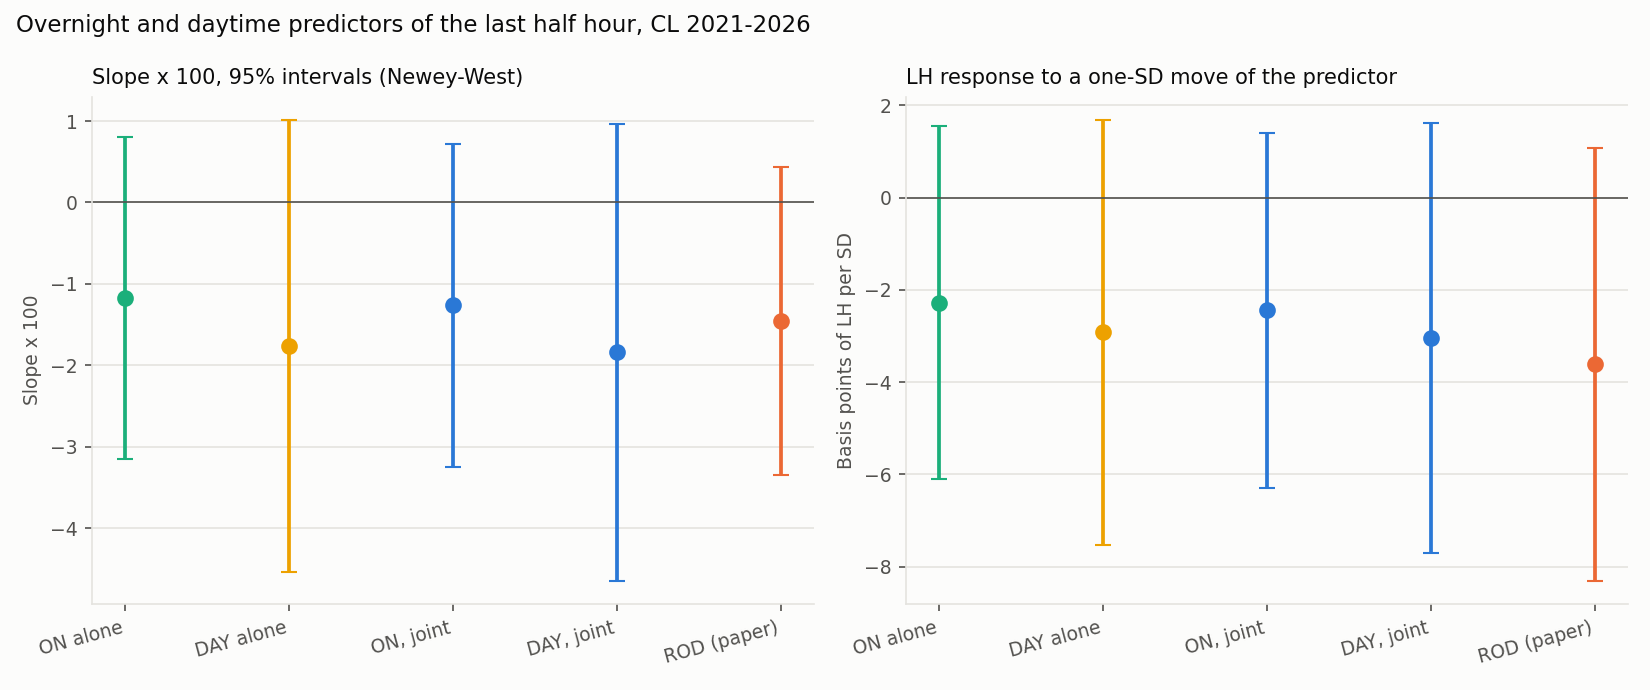
\includegraphics[width=0.8\textwidth]{on_day_slopes.png}
  \begin{itemize}
    \item ON slope $-1.26$ (1.01), DAY slope $-1.84$ (1.43). Difference $0.58$ (1.43).
    \item Every interval includes zero, and the intervals overlap heavily.
  \end{itemize}
\end{frame}

\begin{frame}{Finding 4: high-volatility regimes change nothing measurable}
  \centering
  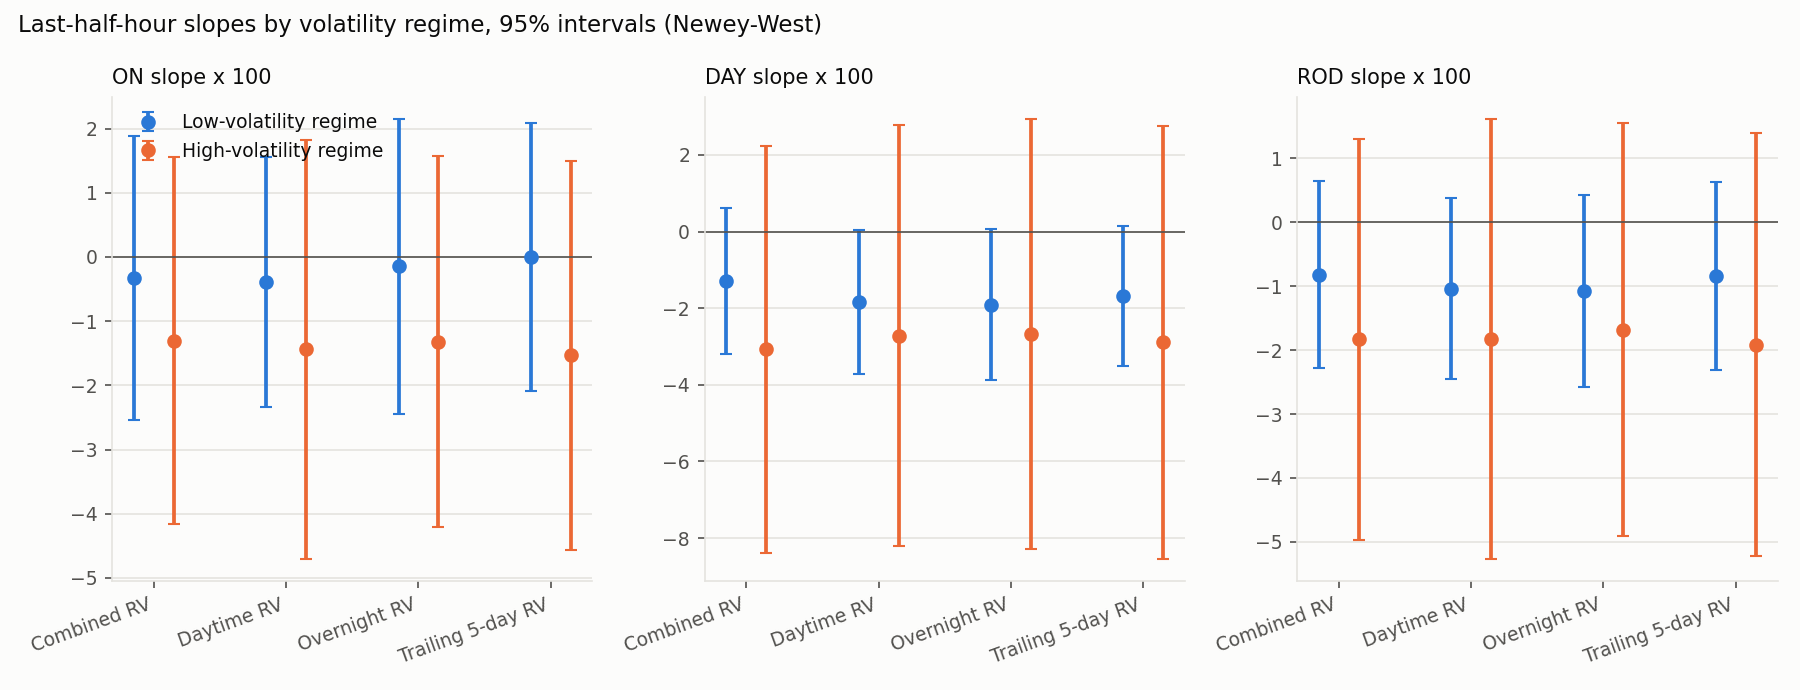
\includegraphics[width=0.85\textwidth]{volatility_regimes_slopes.png}
  \begin{itemize}
    \item High minus low volatility: ON $-1.0$ (1.8), DAY $-1.8$ (2.9). The errors are larger than the shifts.
    \item Realized variance from one-minute returns. High volatility = above the 75th percentile of earlier days.
    \item Four variance definitions give the same picture.
  \end{itemize}
\end{frame}

\begin{frame}{Finding 5: a lead, reversal when ON and DAY agree}
  \begin{columns}[T]
    \begin{column}{0.42\textwidth}
      \small
      \textbf{Agree}: ON and DAY have the same sign (720 days). \textbf{Disagree}: opposite signs (704 days).\\[4pt]
      Paper's strategy return, $\mathrm{sign}(ROD)\cdot LH$:
      \begin{itemize}
        \item Agree: $-4.5$ bp (1.7), the close reverses
        \item Disagree: $+1.9$ bp (1.7)
      \end{itemize}
      Comes almost entirely from 2022 and 2026. Out-of-sample support rests on one day (10 March 2026, see appendix).
    \end{column}
    \begin{column}{0.58\textwidth}
      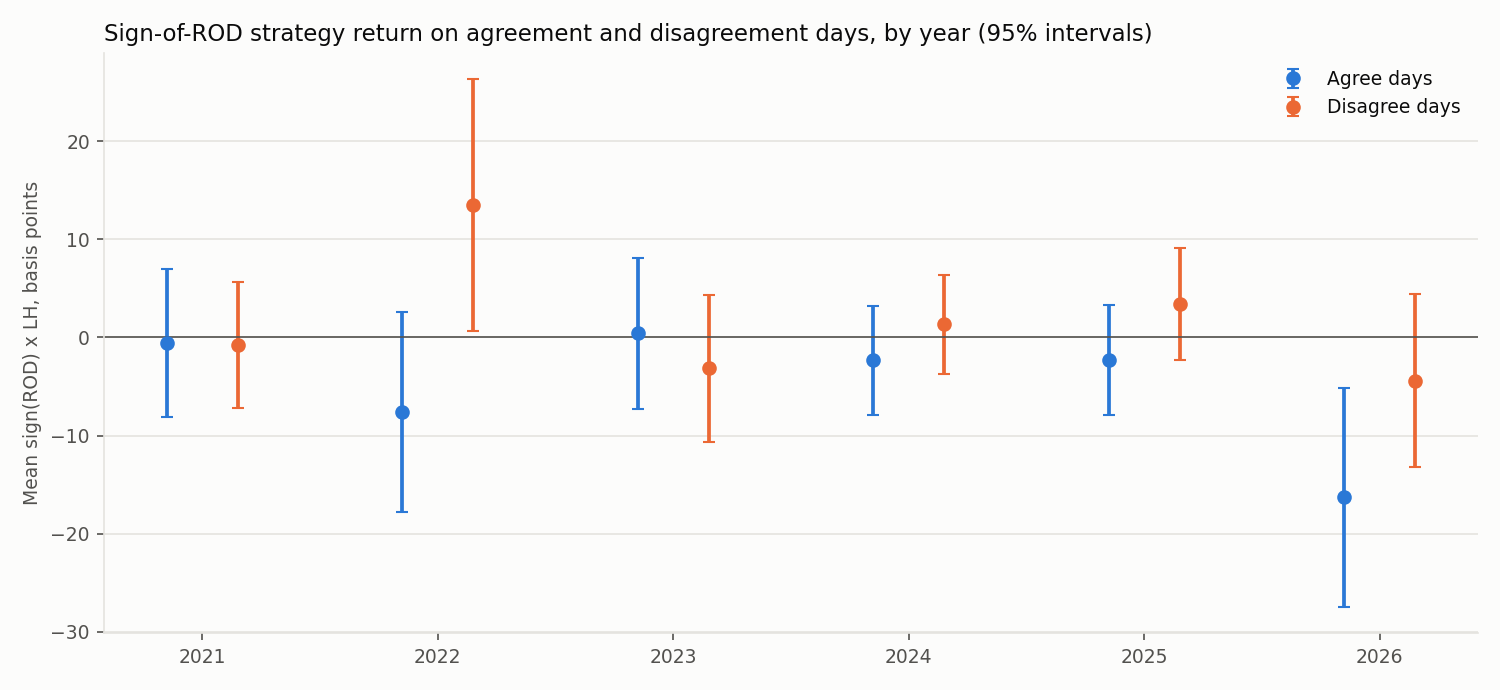
\includegraphics[width=\textwidth]{sign_agreement_by_year.png}
    \end{column}
  \end{columns}
\end{frame}

\begin{frame}{Takeaways and limits}
  \begin{itemize}
    \item The paper's momentum result does not show up in CL after 2020, and it was weak for CL in the original sample too.
    \item The negative slopes are not distinguishable from zero. We do not know why they lean negative.
    \item One market, six years, two crisis episodes, no quote data (spread is a proxy).
    \item \textbf{Next:} a magnitude-based agreement score (beyond our terciles), 2019--2020 minute data, other energy futures.
  \end{itemize}
  \vfill
  \small Reproduce: see the README. No API key needed.
\end{frame}

\appendix
\begin{frame}{Appendix: one day drives much of the signal}
  10 March 2026, Strait of Hormuz closure: ROD $-15.4\%$, then LH $+4.6\%$.
  \begin{itemize}
    \item Dropping it moves the ROD slope from $-1.46$ to $-0.67$ (0.66).
    \item ROD's only positive out-of-sample $R^2$ (0.37\%) becomes $-0.22\%$.
    \item The agreement model's out-of-sample $R^2$ falls from 0.82\% to $-0.47\%$.
  \end{itemize}
  The data is genuine and stays in every baseline. We report results with and without it.
\end{frame}

\begin{frame}{Appendix: the three-predictor regression}
  \[ LH_t = \alpha + \beta_1\, ONFH_t + \beta_2\, M_t + \beta_3\, SLH_t + \varepsilon_t \]
  Slopes $\times 100$ with 95\% intervals. The paper's intervals are implied from its slopes and $t$-statistics.
  \vspace{4pt}
  \begin{center}
  \begin{tabular}{lcc}
    \hline
    & Paper, CL 1987--2020 & Ours, CL 2021--2026\\
    \hline
    ONFH & $2.40\ [-1.80,\ 6.60]$ & $-1.32\ [-3.15,\ 0.51]$\\
    M & $-0.06\ [-3.98,\ 3.86]$ & $-1.94\ [-5.58,\ 1.70]$\\
    SLH & $-13.95\ [-41.57,\ 13.67]$ & $0.38\ [-9.33,\ 10.09]$\\
    \hline
    Adjusted $R^2$ & 1.25\% & 0.46\%\\
    Out-of-sample $R^2$ & $-1.77\%$ & $-1.49\%$\\
    \hline
  \end{tabular}
  \end{center}
  Every post-2020 interval includes zero. SLH is very noisy in both samples.
\end{frame}
\begin{frame}{Appendix H1: overnight vs.\ daytime}
  \small
  Slopes $\times 100$, Newey-West standard errors in parentheses. $n=1{,}436$.
  \begin{center}
  \begin{tabular}{llccc}
    \hline
    Model & Term & Slope (SE) & 95\% interval & OOS $R^2$\\
    \hline
    $LH\sim ON$ & ON & $-1.18$ (1.01) & $[-3.15,\ 0.80]$ & $-0.50\%$\\
    $LH\sim DAY$ & DAY & $-1.76$ (1.42) & $[-4.53,\ 1.02]$ & $0.12\%$\\
    $LH\sim ON+DAY$ & ON & $-1.26$ (1.01) & $[-3.25,\ 0.72]$ & $-0.29\%$\\
     & DAY & $-1.84$ (1.43) & $[-4.64,\ 0.97]$ & \\
    $LH\sim ROD$ (paper) & ROD & $-1.46$ (0.97) & $[-3.35,\ 0.43]$ & $0.37\%$\\
    \hline
  \end{tabular}
  \end{center}
  \begin{itemize}
    \item Equality of slopes: $\beta_{ON}-\beta_{DAY}=0.58$ (1.43), $p=0.69$.
    \item Splitting ROD adds no in-sample fit: adjusted $R^2$ is 0.52\% for both the joint model and ROD.
    \item The daytime part carries the little information there is, mostly in 2026 (DAY slope $-9.7$ (4.0) in 2026).
    \item Dropping 10 March 2026 shrinks both slopes to about $-0.7$.
  \end{itemize}
\end{frame}

\begin{frame}{Appendix H2: volatility regimes}
  \small
  High volatility = realized variance above the upper quartile of earlier days. 336 of 1,186 dates from 2022 qualify, mostly in 2022 and 2026. LH standard deviation is 0.70\% on those days against 0.37\%.
  \begin{center}
  \begin{tabular}{lcccc}
    \hline
    Predictor & Low-vol slope & High-vol slope & High $-$ low (SE), $p$ & Wald $p$\\
    \hline
    ON & $-0.33$ (1.13) & $-1.30$ (1.46) & $-0.97$ (1.84), 0.60 & 0.78\\
    DAY & $-1.29$ (0.97) & $-3.07$ (2.71) & $-1.79$ (2.94), 0.54 & \\
    ROD & $-0.82$ (0.75) & $-1.83$ (1.60) & $-1.01$ (1.77), 0.57 & \\
    \hline
  \end{tabular}
  \end{center}
  \begin{itemize}
    \item Daytime, overnight and trailing 5-day variance regimes give the same picture. None of the eight interaction $p$-values is below 0.41.
    \item Out of sample, adding regime terms to $LH\sim ON+DAY$ lowers OOS $R^2$ from 0.35\% to between $-0.6\%$ and $-1.2\%$, mostly in March 2026.
    \item Without 10 March 2026 the high-regime differences shrink to $-0.07$ and $+0.70$.
  \end{itemize}
\end{frame}

\begin{frame}{Appendix H3: what ``agree'' and ``disagree'' mean}
  \begin{columns}[T]
    \begin{column}{0.56\textwidth}
      \centering
      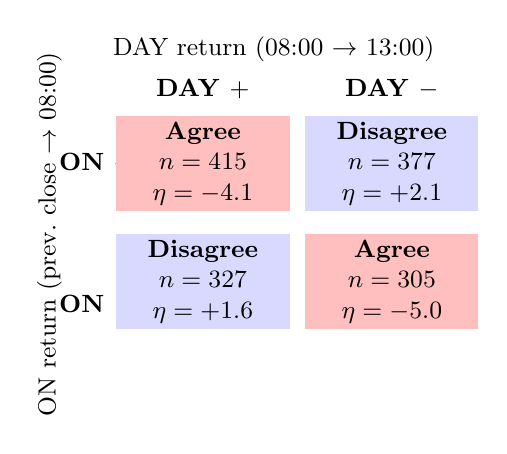
\begin{tikzpicture}[x=1cm,y=1cm]
        \node[font=\small] at (2.1,3.55) {DAY return (08:00 $\to$ 13:00)};
        \node[font=\small\bfseries] at (1.2,3.05) {DAY $+$};
        \node[font=\small\bfseries] at (3.6,3.05) {DAY $-$};
        \node[font=\small,rotate=90] at (-0.75,1.2) {ON return (prev.\ close $\to$ 08:00)};
        \node[font=\small\bfseries] at (-0.15,2.1) {ON $+$};
        \node[font=\small\bfseries] at (-0.15,0.3) {ON $-$};
        \fill[red!25]    (0.1,1.5) rectangle (2.3,2.7);
        \fill[red!25]    (2.5,0.0) rectangle (4.7,1.2) ;
        \fill[blue!15]   (2.5,1.5) rectangle (4.7,2.7);
        \fill[blue!15]   (0.1,0.0) rectangle (2.3,1.2);
        \node[align=center,font=\small] at (1.2,2.1) {\textbf{Agree}\\$n=415$\\$\eta=-4.1$};
        \node[align=center,font=\small] at (3.6,0.6) {\textbf{Agree}\\$n=305$\\$\eta=-5.0$};
        \node[align=center,font=\small] at (3.6,2.1) {\textbf{Disagree}\\$n=377$\\$\eta=+2.1$};
        \node[align=center,font=\small] at (1.2,0.6) {\textbf{Disagree}\\$n=327$\\$\eta=+1.6$};
      \end{tikzpicture}
    \end{column}
    \begin{column}{0.44\textwidth}
      \small
      \textbf{Agree}: ON and DAY have the same sign, so the day moved one way.\\[4pt]
      \textbf{Disagree}: opposite signs, so the overnight move was partly undone.\\[6pt]
      $\eta=\mathrm{sign}(ROD)\cdot LH$, in basis points:
      \begin{itemize}
        \item $\eta>0$: the close \emph{continues} the day's direction (momentum)
        \item $\eta<0$: the close \emph{reverses} it
      \end{itemize}
    \end{column}
  \end{columns}
  \vspace{4pt}
  \small Example: ON $+1\%$ and DAY $+0.8\%$ is an agreement day. Momentum predicts LH goes up. On agreement days the close tends to fall instead. Both signs are known at 13:00.
\end{frame}

\begin{frame}{Appendix H3: agreement between ON and DAY}
  \small
  Strategy return $\eta=\mathrm{sign}(ROD)\cdot LH$ in basis points, Newey-West standard errors. 12 days with a zero return are set aside.
  \begin{center}
  \begin{tabular}{lcccc}
    \hline
    Group & $n$ & Mean $LH$ (SE) & $\eta$ (SE) & Hit rate\\
    \hline
    ON$+$/DAY$+$ & 415 & $-4.11$ (1.94) & $-4.11$ (1.94) & 0.477\\
    ON$-$/DAY$-$ & 305 & $5.00$ (3.01) & $-5.00$ (3.01) & 0.470\\
    ON$+$/DAY$-$ & 377 & $-3.69$ (2.30) & $2.10$ (2.34) & 0.515\\
    ON$-$/DAY$+$ & 327 & $-1.07$ (2.42) & $1.62$ (2.39) & 0.476\\
    \hline
    Agree $-$ disagree & 1,424 & & $-6.36$ (2.34), $p=0.007$ & \\
    \hline
  \end{tabular}
  \end{center}
  \begin{itemize}
    \item $LH=\alpha+\beta ROD+\gamma Agree+\delta ROD{\cdot}Agree$: $\hat\beta=2.29$ (1.25), $\hat\delta=-4.93$ (1.61). The slope is about $-2.64$ on agreement days.
    \item Year by year: $-21$ (8) bp in 2022 and $-12$ (7) in 2026, within $\pm6$ of zero elsewhere. Without both years: $-1.4$ (2.3).
    \item OOS $R^2$ rises from 0.43\% to 0.82\% ($p=0.051$) but is $-0.47\%$ without 10 March 2026.
  \end{itemize}
\end{frame}

\end{document}
